\chapter{Finalisierung}

\section{Nachbearbeitung und Zusammenbau}
Nach dem Druck der Teile müssen diese Nachbearbeitet werden. Hierzu zählt das Entfernen des Rafts, des Stützmaterials und eventueller Druckfehler. Werden Schrauben verwendet müssen für diese ggf. Gewinde geschnitten werden, was bei dem gegebenen Projekt jedoch nicht nötig war.

Anschließend kann das Projekt anhand der Bauanleitung aufgebaut werden.

\begin{figure}[h]
  \centering
  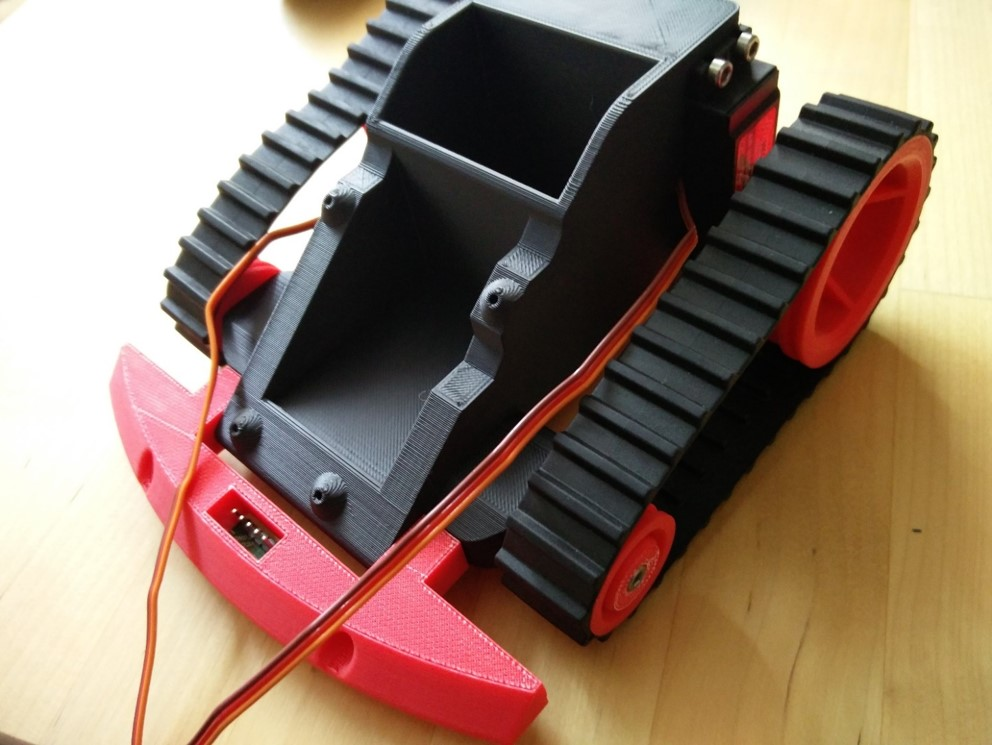
\includegraphics[width=12cm]{kapitel5/built}
  \caption{Alle Teile sind verbaut}
  \label{Kap4:Built}
\end{figure}

Wenn alle Teile verbaut sind, kann die Elektronik anhand des Schaltplans aufgebaut werden.

\begin{figure}[h]
  \centering
  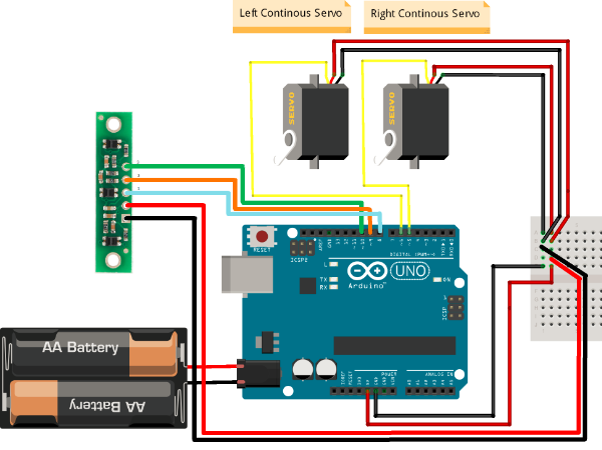
\includegraphics[width=12cm]{kapitel5/schaltung}
  \caption{Darstellung der Schaltung}
  \label{Kap4:Schaltung}
\end{figure}

\clearpage

\section{Fertiges Projekt}
Mit dem Abschluss aller Schritte ist auch das Projekt abgeschlossen.

\begin{figure}[h]
  \centering
  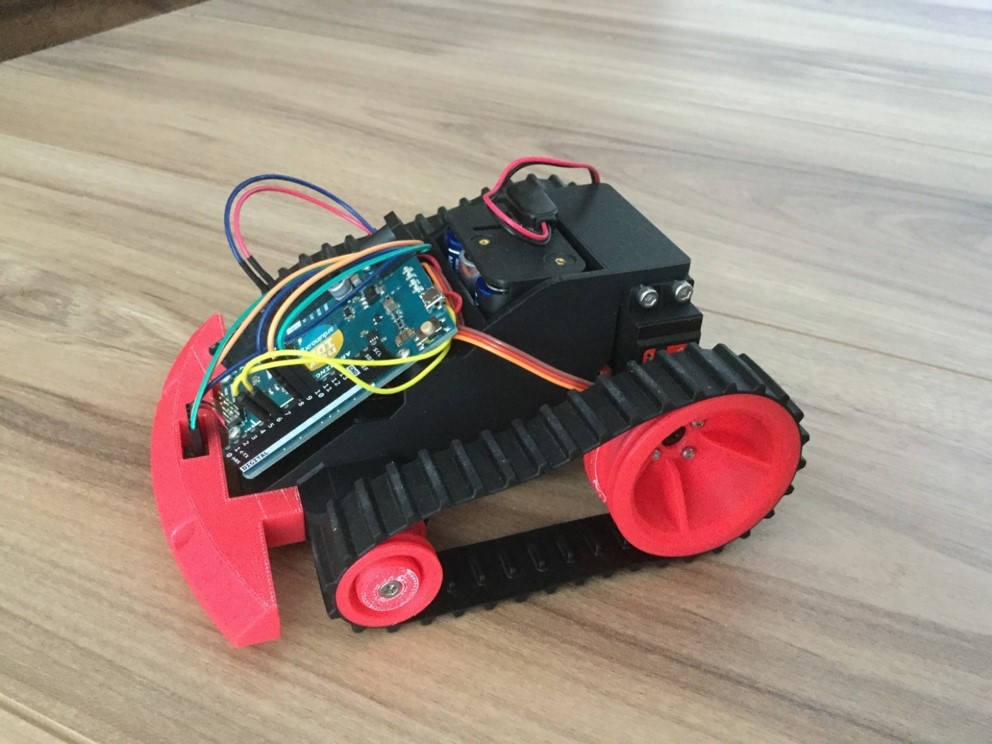
\includegraphics[width=14cm]{kapitel5/final}
  \caption{Das Projekt ist abgeschlossen}
  \label{Kap4:Final}
\end{figure}